\documentclass[bare_jrnl_transmag]{subfiles}
\begin{document}
\subsection{Limitations}
From the results of the filter, it is apparent that, while performing better than a pure dead-reckoning approach, the Kalman filter exhibits drift in its position estimation. Figure \ref{fig:dead_reackoning} shows the results of an inertial dead-reckoning approach on the training dataset, demonstrating the improvement offered with the vision-based fusion. The RSME of the dead-reckoning approach is 7.01, 10.08, and 0.91 meters.

\begin{figure}[H]
    \centering
    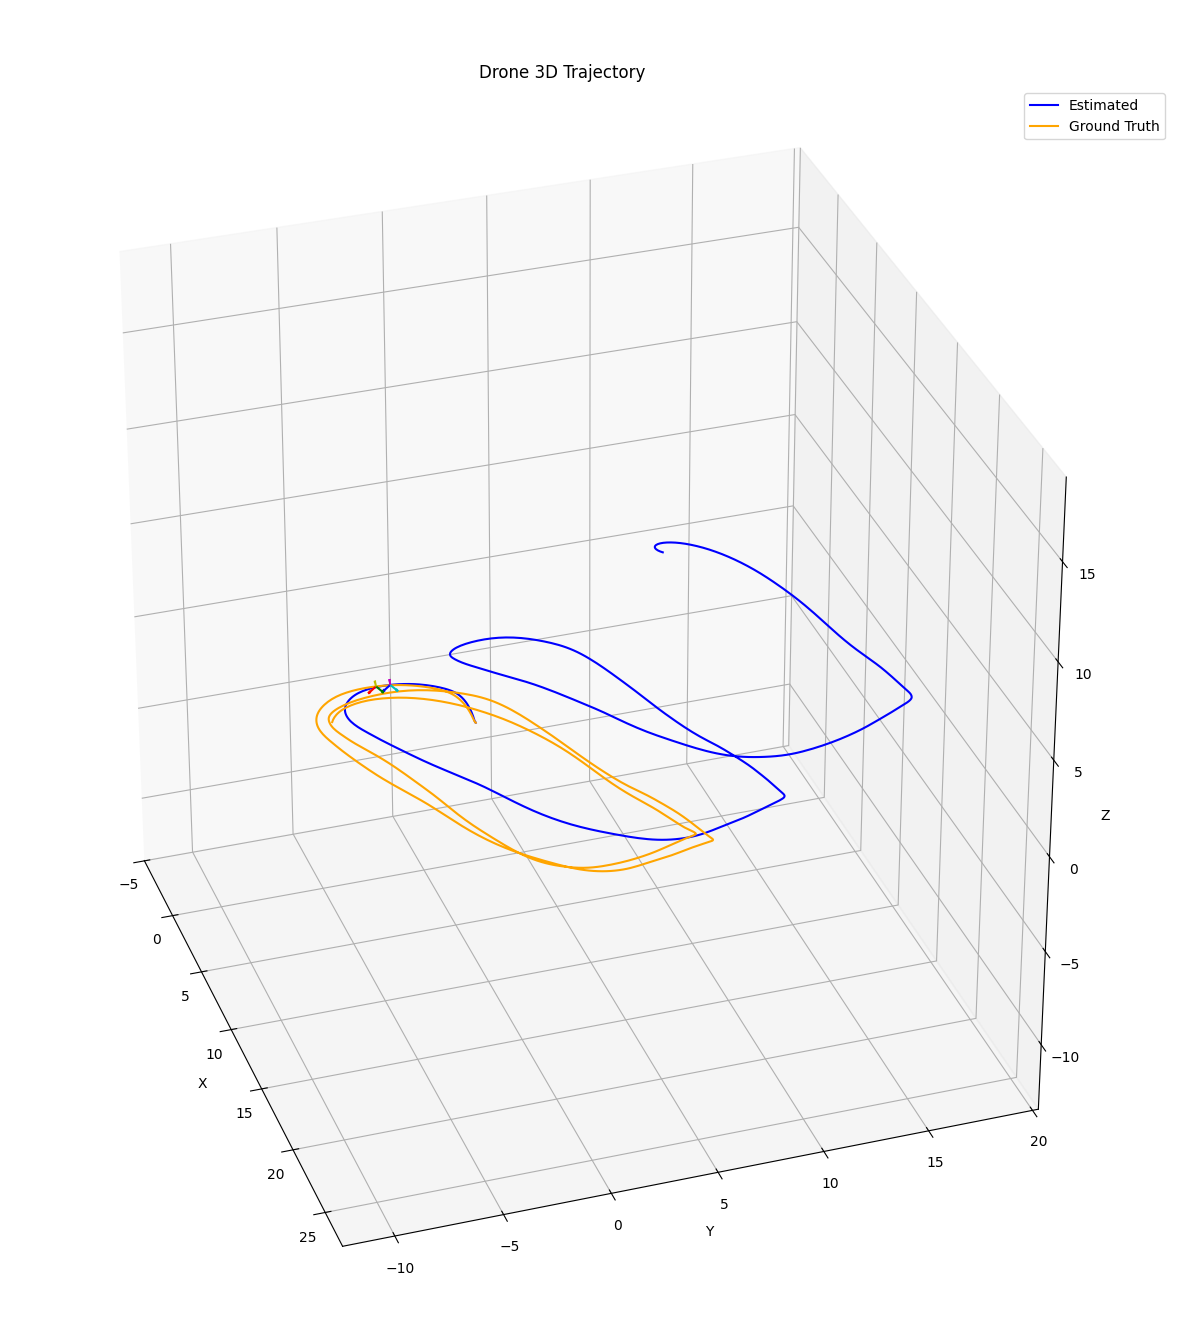
\includegraphics[width=0.8\linewidth]{figures/dead_reckoning_results_training.png}
    \caption{Dead-reckoning results comparing the ground-truth pose of the drone to the estimated pose on the training dataset.}
    \label{fig:dead_reackoning}
\end{figure}

The above figure shows the significant amount of drift that results from a pure dead-reckoning approach in the X/Y plane. The Kalman filter is able to reduce this drift significantly, but it is still present. While the orientation estimation is quite accurate, the Madgwick filter has no way of correcting for yaw drift in the absence of another sensor (ex: magnetometer). As a result,a poor yaw estimate will cause the position estimation to drift, especially as the motion model directly integrates acceleration measurements in the estimated body frame. 


\end{document}